Climate change and carbon neutrality have garnered widespread global attention. The significant amount of carbon emissions during electricity production underscores the importance of achieving low-carbon electricity production as a solution to these pressing challenges.
In recent years, wind and solar energy have emerged as promising sources of sustainable electricity. However, the fluctuation patterns of these sources are highly variable, making it challenging to accurately predict their power generation capacity over the long term.
This presents a major challenge for existing power scheduling systems that rely on reliable long-term forecasts and day-ahead calculation, potentially leading to suboptimal or infeasible solutions, including renewable curtailments and blackouts~\cite{enwiki:1103904998,bialek2020does}.

Traditionally, power system operators perform the day-ahead scheduling (DAS) program to calculate power generation schedules~\cite{wood2013power}. 
The DAS program consists of unit commitment (UC) and economic dispatch (ED) as depicted in Fig.\ref{fig:das-vs-rts}(A). 
UC aims at optimizing the combinations of operating power generators to reduce operational costs while maintaining a sufficient power supply. It is an NP-hard problem since it optimizes high-dimensional continuous and integer variables (startup/shutdown of thermal generators) for many time steps~\cite{bendotti2019complexity}.
It is typically solved using the time-consuming mixed integer programming (MIP) method~\cite{bhardwaj2012unit,jabr2012tight}, which could only be calculated a long time in advance. This makes UC heavily rely on accurate forecasts while the day-ahead forecasts of renewable generation are presently unreliable. 
Alternative methods, including reinforcement learning~\cite{de2021applying,de2022reinforcement,ajagekar2022deep}, however, have still been proposed as offline control, nor considered complex network constraints such as transmission line capacity, which is infeasible in actual scheduling. 
On the other hand, ED is usually modeled as a convex optimization problem and can be solved by the interior point and dual methods~\cite{jabr2002primal, olofsson1995linear,sun1984optimal}, but these methods still encounter problems of convergence and computational speed in the face of AC power flow models, in which ED turns into a non-convex problem.
Reinforcement learning methods are also studied to solve ED problems in real-time, while \cite{zhou2020data,zhou2021deep,woo2020real} uses out-of-date algorithms and power grids with a low proportion of renewable energy, which does not accord with future grid development. These RL methods did not consider complex operational constraints such as reactive power limitation and line transmission capacity either.
In general, studying UC or ED alone is inadequate to solve the challenges faced by the power system today.
% How to execute joint optimization at a finer time resolution remains a topic of ongoing research.


The limitations of existing scheduling methods have prompted the adoption of hardware upgrades as alternative solutions, which aimed at increasing flexibility resources, including thermal unit retrofits and energy storage constructions. However, these upgrades come at significant investments. Additionally, if the retrofitted thermal units operate outside of their design specifications, it can lead to elevated carbon emissions and increased costs per megawatt power~\cite{chen2021flexible}. Electrochemical energy storage options, such as batteries, are criticized for their high cost, limited lifespan, and environmental concerns. Physical-based energy storage technologies, such as pumped hydroelectricity and compressed air storage, are also subject to site availability and long construction cycles. Therefore, relying solely on hardware upgrades for enhancing future power scheduling is not a practical and economically viable solution. 


We propose to reform the power scheduling system through joint optimization of the above two subproblems with finer time resolutions, referred to as the Real-Time Scheduling (RTS) problem, as demonstrated in Fig.\ref{fig:das-vs-rts}(B). 
This is because recent advancements in deep learning have significantly improved the accuracy of ultra-short-term renewable generation forecasts~\cite{wu2021ultra,tawn2022review}.
The integration of ultra-short-term forecasts enables the transformation of scheduling grids with renewable energy into a deterministic problem within a limited time horizon.
However, traditional optimization algorithms face challenges in generating schedule plans within this short time frame. 
Therefore, there is a need for the development of innovative scheduling algorithms and a shift towards a computationally efficient framework, which is capable of real-time optimization of unit commitment and economic dispatch simultaneously.


In contrast to optimizing UC and ED separately, we take a drastically different technical approach to real-time joint optimization and take all system operational constraints into consideration.
We propose to take advantage of reinforcement learning (RL) to solve the problem in real-time by shifting the intensive computational burden of traditional optimization algorithms to an offline training process. 
RL has shown its capabilities to solve complex control tasks while remaining computationally efficient\cite{mnih2015human,lillicrap2015continuous,haarnoja2018soft,schulman2017proximal,silver2016mastering}. Some aspects of power systems, such as full-fledged simulation and wide-spread smart measurements, are suitable for RL's applications.
However, we find that the most widely used RL algorithms, such as Deep Deterministic Policy Gradient (DDPG)\cite{lillicrap2015continuous}, Soft Actor-Critic (SAC)\cite{haarnoja2018soft}, and Proximal Policy Optimization (PPO)\cite{schulman2017proximal} are unable to achieve satisfactory results. As a result, we developed a look-ahead scheduling RL method called GridZero, built upon the state-of-the-art AlphaGo series' work, which excels in complex board games~\cite{silver2016mastering,li2018alphago,silver2017mastering,schrittwieser2020mastering}, robotic control~\cite{hubert2021learning}, scientific discovery~\cite{fawzi2022discovering}, and video compression~\cite{mandhane2022muzero}.
The choice of this search plus deep learning framework for solving the RTS task is based on the common feature between power scheduling and Go games, which both require the look-ahead search for future possible situations. The search method in the AlphaGo series has been demonstrated to produce robust and conservative policies, which are critical for power dispatching, as security is the first criterion of the power grid. 


The simulation results of the real power grid demonstrate the efficacy of our proposed method in addressing the major challenges hindering the widespread adoption of renewable energy. Specifically, our method enables fast scheduling, reduces renewable generation curtailment, eliminates load shedding, and minimizes the need for expensive hardware upgrades. In the test scenario with a high share of renewable generation, our method reduced renewable generation curtailment by 79\% and eliminated load shedding - issues that are commonly encountered in DAS due to unreliable forecasts. By executing control at finer time resolution, our method conserves the cost of hardware upgrades, which would have required an upgraded capacity of 20\% of the total installed capacity, equating to a minimum investment of 60 million dollars. This amount of savings is sufficient to build 14 100-MW coal-fired power plants. In conclusion, our RL-based method guarantees stable and efficient real-time scheduling in power systems with high renewable energy penetration.


\begin{figure}[h]
  \centering
  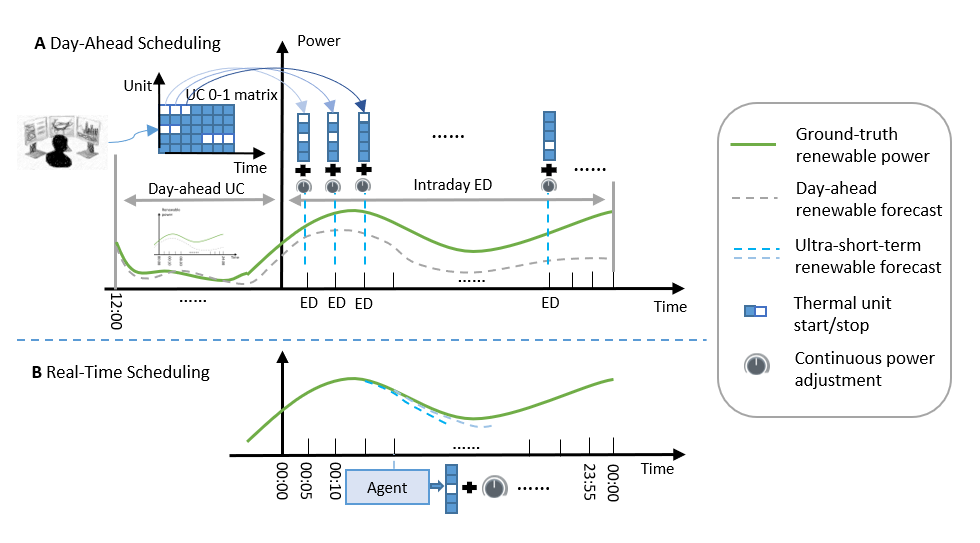
\includegraphics[width=0.9\linewidth]{fig/das_rts.png}
  \caption{\textbf{DAS vs RTS-GridZero.}
  \textbf{(A) Day-Ahead Scheduling.} DAS performs day-ahead unit commitment to determine the startup/shutdown schedule of thermal generators according to the future 36 hours forecasts, including load and renewable generation. However, the forecasts of renewable generation will become more and more unreliable as the prediction period grows. This introduces errors in the optimization process of the unit commitment, resulting in an unreasonable 0-1 matrix output. Although the coming intraday economic dispatch can partially mitigate the impacts of errors, renewable curtailment and load shedding will occur when the error scale is large.
  \textbf{(B) Real-Time Scheduling.} Conversely, RTS adjusts power generators with a finer time resolution. The control interval is the minute level rather than the day level of the conventional day-ahead scheduling. This is achieved through precise ultra-short-term forecasts and data-driven, computation-efficient reinforcement learning algorithms. Within the narrow period of accurate ultra-short-term forecasts, the scheduling problem is back to a deterministic control problem. The RL agent controls the output power and startup/shutdown of generators simultaneously, corresponding to joint optimization of unit commitment and economic dispatch. Furthermore, our proposed GridZero is capable of look-ahead scheduling for the incoming decision scenarios.
  } 
  \label{fig:das-vs-rts}
\end{figure}

\begin{figure}[h]
  \centering
  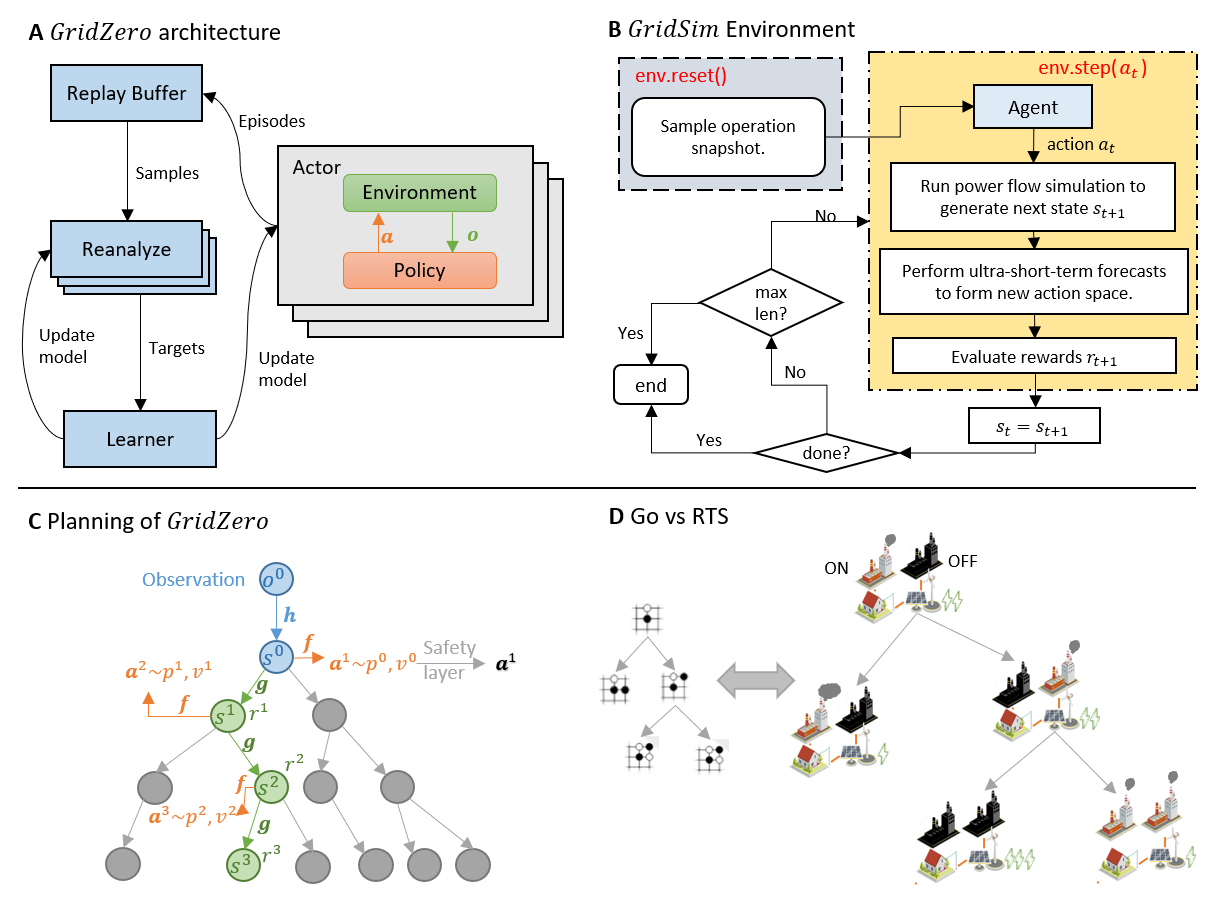
\includegraphics[width=0.9\linewidth]{fig/nature_fig6.png}
  \caption{\textbf{Illustration of GridZero.}
  \textbf{(A) Architecture.}  
  Actors interact with GridSim to collect state transitions which are then stored in a replay buffer. The replay buffer feeds data to reanalyze to make targets for the learner.
  \textbf{(B) Flow chart of power scheduling RL environment.} 
  GridSim simulates the next state through power flow computation, performs forecasts for load and renewable generation capacity, and calculates the reward.
  % includes components such as renewable and load prediction, power flow simulation, and reward calculation.
  \textbf{(C) Look-ahead scheduling.} GridZero grows a search tree, with the observation $o$ encoded as root hidden state $s$ by the representation network $h$. During each simulation, the algorithm descends to a leaf node along the most promising path and adds a new leaf. The dynamics network $g$ estimates the hidden state $s$ and reward $r$ of each new node, while the prediction network $f$ provides the value $v$ and policy $p$. The action is selected from the root visit distribution and may be adjusted to ensure safety.
  \textbf{(D) Go vs RTS}. AlphaGo's success in the game of Go benefits from the look-ahead search for both sides' actions. The search mechanism is beneficial for the agent to search for a future step that is far beyond what a human can think about and to make the most rational decision. This idea is also suited for power scheduling since the operators need to simulate multi-step future scenarios and make the most reasonable scheduling plan. 
  } 
  \label{fig:nature_fig1}
\end{figure}


\subsection*{Real-time scheduling as an RL problem}
Optimization-based methods are time-consuming, resulting in a reliance that traditional scheduling methods can only be performed through prior computation.
This can lead to scheduling results susceptible to errors in day-ahead forecasts of renewable generation. 

Real-time scheduling (RTS) addresses this challenge by utilizing precise ultra-short-term forecasts to solve a nearly deterministic problem. 
Reinforcement learning (RL) is a compatible solution for RTS, as it shifts the time-intensive computation to the offline training process, exhibiting the ability to resolve other complex control tasks~\cite{silver2016mastering,lillicrap2015continuous,schulman2017proximal,degrave2022magnetic,fawzi2022discovering,mandhane2022muzero}.
In this study, the RTS problem is reformulated as a sequential Markov decision process (MDP). 
The proposed scheduling MDP incorporates ultra-short-term forecasts as components of the observation. It considers all operational constraints and optimization objectives of the power system operation in the reward function, guiding the agent to improve the scheduling objectives while adhering to operational constraints. 
This MDP serves as a foundation for deploying computationally efficient RL algorithms.

The proposed RL-based RTS framework is illustrated in Fig.\ref{fig:nature_fig1}. Our approach encompasses two major phases. Initially, the RTS issue is represented as a Markov Decision Process (MDP) and an RL environment, referred to as GridSim, is constructed. Subsequently, a look-ahead scheduling RL agent is introduced that interacts with GridSim to learn near-optimal control policies through a systematic search and training procedure.

In the initial phase, 
the MDP and Gridsim environment are modeled as follows:
\begin{enumerate}[label=(\arabic*)]
    \item Observations encode the grid's operational states, including generator power outputs, load consumption power, line transmission currents, bus voltages, etc. Observations also include the next-step prediction of renewable maximum power and load consumption.
    \item Actions are designed as concatenations of generator active power outputs' continuous adjustments and discrete unit startup/shutdowns, 
    which aims to optimize the economic dispatch and unit commitment simultaneously. Furthermore, renewable generators do not always output full power. Their power setpoint range is $[0, \overline{\text{p}^t}]$ where $\overline{\text{p}^t}$ is the maximum power of renewable generators at step $t$. Renewable curtailment is the difference between the maximum power and the actual power of renewable generators.
    \item State transitions represent the conversion to the next power system steady state, and they are modeled in AC power flow models and simulated through a professional power flow analysis program, which solves the power flow equations via the Newton-Raphson method. 
    \item The reward is a scalar function that measures the grid's current state under the criteria of specific constraints and objectives. It also penalizes actions that lead to undesirable states that violate operational constraints.
\end{enumerate}


In the second phase, an RL algorithm called GridZero is designed to make better use of the look-ahead search's benefits in solving the RTS problem. GridZero interacts with GridSim and accumulates state transition data to develop policies.
The architecture of tree search combined with deep neural networks delivers more stable policy improvements compared to commonly utilized model-free RL methods such as\cite{lillicrap2015continuous,haarnoja2018soft}. This enables GridZero to attain satisfactory scheduling performances in the RTS task. 
The capability comparison between GridZero and conventional methods is presented in Table.\ref{tab:capability}. GridZero represents a groundbreaking RL-based method that not only satisfies the real-time requirement and utilizes ultra-short-term forecasting but also possesses the ability to plan for future scenarios.


\begin{table}[h]
\centering
\caption{Comparisons of DAS, Model-free RL, and GridZero. GridZero achieves look-ahead scheduling, utilization of ultra-short-term forecasts, and real-time scheduling simultaneously.}
% \begin{tiny}
\begin{tabular}{cccc}
    \toprule
      & DAS & Model-free RL & GridZero \\
    \midrule
    Look-ahead scheduling & \CheckmarkBold & \XSolidBold & \CheckmarkBold \\
    Ultra-short-term forecasts & \XSolidBold & \CheckmarkBold & \CheckmarkBold \\
    Real-time decision-making & \XSolidBold & \CheckmarkBold & \CheckmarkBold \\
    \bottomrule
  \end{tabular}
% \end{tiny}
  \label{tab:capability}
\end{table}

As depicted in Fig.\ref{fig:nature_fig1}(C), a systematic search process characterized by a growing search tree, is employed to find a carefully selected action candidate. This process evaluates the grid scheduling actions by simulating how the grid will change after the proposed actions, facilitated by the dynamic function. Through a hybrid sampling process, the policy function proposes action candidates to narrow the search process to promising future scenarios.
The value function then assesses the preference of states encountered during the search process, by estimating the discounted future reward. The UCB score, a combination of value prediction and node visited number, balances exploration and exploitation, thus guiding the selection process in the tree search. Intuitively, the search process could avoid the case when the current operation is valid but leads to future grid states that are hard to handle. It is reminiscent of how an experienced power grid manager operates the grid, as they intuitively know some good candidate controlling options according to their past experience, and then they validate the operation by further simulations. 


Meanwhile, we propose a safety layer to prevent the RL agent from causing destructive consequences due to unrestricted exploration in this risk-sensitive task.
Purely random explorations can lead to severe consequences, as randomly setting the generators' power outputs cannot guarantee the basic load-generation balance.  
This is particularly concerning in power systems because any violations of this constraint can result in blackouts or even system failures\cite{enwiki:1103904998,bialek2020does}.
To simulate real scenarios, GridSim implemented such violations of power balancing as immediate episode terminations, which makes it difficult for agents to continuously interact with GridSim while exploring without limit.
Additionally, the temporal varieties of renewable generation make the action space change over time. 
To satisfy this time-varying power balance constraint, the safety layer provides a feasible solution space, which enables the RL agent to explore safely in it. 
Such a safety layer is common in many other similar tasks with high-security requirements\cite{shao2022safety,chitta2022transfuser}.
